\documentclass{article}

% -----------------------------
% Packages
% -----------------------------
\usepackage{fancyhdr}
\usepackage{extramarks}
\usepackage{amsmath}
\usepackage{amsthm}
\usepackage{amsfonts}
\usepackage{tikz}
\usepackage[plain]{algorithm}
\usepackage{algpseudocode}
\usepackage{amssymb}
\usepackage{graphicx}

\usetikzlibrary{automata,positioning}

% -----------------------------
% Basic Document Settings
% -----------------------------
\topmargin=-0.45in
\evensidemargin=0in
\oddsidemargin=0in
\textwidth=6.5in
\textheight=9.0in
\headsep=0.25in

\linespread{1.1}

\pagestyle{fancy}
\lhead{\hmwkAuthorName}
\chead{\hmwkClass: \hmwkTitle}
\rhead{}
\lfoot{\lastxmark}
\cfoot{\thepage}

\renewcommand\headrulewidth{0.4pt}
\renewcommand\footrulewidth{0.4pt}

\setlength\parindent{0pt}

% -----------------------------
% Problem Section Helpers
% -----------------------------
\newcommand{\enterProblemHeader}[1]{
  \nobreak\extramarks{}{Problem \arabic{#1} continued on next page\ldots}\nobreak{}
  \nobreak\extramarks{Problem \arabic{#1} (continued)}{Problem \arabic{#1} continued on next page\ldots}\nobreak{}
}

\newcommand{\exitProblemHeader}[1]{
  \nobreak\extramarks{Problem \arabic{#1} (continued)}{Problem \arabic{#1} continued on next page\ldots}\nobreak{}
  \stepcounter{#1}
  \nobreak\extramarks{Problem \arabic{#1}}{}\nobreak{}
}

\setcounter{secnumdepth}{0}
\newcounter{partCounter}
\newcounter{homeworkProblemCounter}
\setcounter{homeworkProblemCounter}{1}
\nobreak\extramarks{Problem \arabic{homeworkProblemCounter}}{}\nobreak{}

% -----------------------------
% Theorem env (optional)
% -----------------------------
\newtheorem*{theorem}{Theorem}

% -----------------------------
% Homework Problem Environment
%   Usage:
%   \begin{homeworkProblem}            % auto-number
%     % Your answer here
%   \end{homeworkProblem}
%
%   \begin{homeworkProblem}[7]         % set problem number to 7
%     % Your answer here
%   \end{homeworkProblem}
% -----------------------------
\newenvironment{homeworkProblem}[1][-1]{
  \ifnum#1>0
    \setcounter{homeworkProblemCounter}{#1}
  \fi
  \section{Problem \arabic{homeworkProblemCounter}}
  \setcounter{partCounter}{1}
  \enterProblemHeader{homeworkProblemCounter}
}{
  \exitProblemHeader{homeworkProblemCounter}
}

% -----------------------------
% Homework Details (EDIT THESE)
% -----------------------------
\newcommand{\hmwkTitle}{Homework \ 2}
\newcommand{\hmwkClass}{CS 4262}
\newcommand{\hmwkClassInstructor}{Prof. Dr. Thomas Beckers}
\newcommand{\hmwkAuthorName}{\textbf{Joseph Quinn}}

% -----------------------------
% Title
% -----------------------------
\title{
  \vspace{2in}
  \textmd{\textbf{\hmwkClass:\ \hmwkTitle}}\\
  \vspace{0.1in}\large{\textit{\hmwkClassInstructor\ }}
  \vspace{3in}
}
\author{\hmwkAuthorName}
\date{}

% -----------------------------
% Convenience Macros (optional)
% -----------------------------
\renewcommand{\part}[1]{\textbf{\large Part \Alph{partCounter}}\stepcounter{partCounter}\\}

% Algorithms
\newcommand{\alg}[1]{\textsc{\bfseries \footnotesize #1}}

% Calculus
\newcommand{\deriv}[1]{\frac{\mathrm{d}}{\mathrm{d}x} (#1)}
\newcommand{\pderiv}[2]{\frac{\partial}{\partial #1} (#2)}
\newcommand{\dx}{\mathrm{d}x}

% Statistics
\newcommand{\E}{\mathrm{E}}
\newcommand{\Var}{\mathrm{Var}}
\newcommand{\Cov}{\mathrm{Cov}}
\newcommand{\Bias}{\mathrm{Bias}}

% Proof step (for aligned derivations)
\newcommand{\step}[2]{& #1 & & \text{#2} \\}

% Solution header (optional)
\newcommand{\solution}{\textbf{\large Solution}}

% -----------------------------
% Document
% -----------------------------
\begin{document}

\maketitle
\pagebreak

\begin{homeworkProblem}
	\subsection*{1.1 The Primal form of soft margin SVM}
	\[
		\min_{w,b,\{\xi_i\}} \quad w^T w + C \sum_i \xi^{(i)}
		\;\; \text{s.t.} \;\; y^{(i)} \big(w^T x^{(i)} + b\big) \;\geq\; 1 - \xi^{(i)}, \;\; \forall i,
		\;\; \xi^{(i)} \;\geq\; 0, \quad \forall i
	\]
	\subsection*{1.2 Dual form of the soft-margin SVM}

	We introduce multipliers $\alpha_i \geq 0$ for the margin constraints and $\mu_i \geq 0$ for the $\xi_i \geq 0$ constraints. The Lagrangian is

	\[
		\begin{aligned}
			\mathcal{L}(w,b,\xi;\alpha,\mu)
			 & = \frac12 \lVert w \rVert_2^2 + C\sum_{i=1}^n \xi_i
			- \sum_{i=1}^n \alpha_i \Big( y_i (w^\top x_i + b) - 1 + \xi_i \Big)
			- \sum_{i=1}^n \mu_i \xi_i .
		\end{aligned}
	\]

	Stationary conditions:
	\begin{align*}
		\frac{\partial \mathcal{L}}{\partial w}     & = w - \sum_{i=1}^n \alpha_i y_i x_i = 0
		\quad \Rightarrow \quad w = \sum_{i=1}^n \alpha_i y_i x_i ,                           \\
		\frac{\partial \mathcal{L}}{\partial b}     & = - \sum_{i=1}^n \alpha_i y_i = 0
		\quad \Rightarrow \quad \sum_{i=1}^n \alpha_i y_i = 0 ,                               \\
		\frac{\partial \mathcal{L}}{\partial \xi_i} & = C - \alpha_i - \mu_i = 0
		\quad \Rightarrow \quad \mu_i = C - \alpha_i .
	\end{align*}

	Since $\mu_i \geq 0$, we obtain the constraint
	\[
		0 \leq \alpha_i \leq C .
	\]

	Substituting $w$ and constraints into $\mathcal{L}$ gives
	\[
		W(\alpha) = \sum_{i=1}^n \alpha_i
		- \frac12 \sum_{i=1}^n \sum_{j=1}^n \alpha_i \alpha_j y_i y_j \, x_i^\top x_j .
	\]

	The dual is therefore

	\[
		\begin{aligned}
			\max_{\alpha \in \mathbb{R}^n} \quad &
			\sum_{i=1}^n \alpha_i - \frac12 \sum_{i=1}^n \sum_{j=1}^n \alpha_i \alpha_j y_i y_j \, x_i^\top x_j \\
			\text{s.t.} \quad                    & 0 \leq \alpha_i \leq C, \quad i=1,\dots,n,                   \\
			                                     & \sum_{i=1}^n \alpha_i y_i = 0 .
		\end{aligned}
	\]

	Bias $b$ can be recovered from any support vector $x_s$ with $0 < \alpha_s < C$:
	\[
		b = y_s - \sum_{j=1}^n \alpha_j y_j x_j^\top x_s .
	\]

	\subsection*{1.3 Kernelized soft-margin SVM}

	We replace the inner product $x_i^\top x_j$ with a kernel $k(x_i,x_j) = \langle \phi(x_i),\phi(x_j)\rangle$. The dual becomes

	\[
		\begin{aligned}
			\max_{\alpha} \quad & \sum_{i=1}^n \alpha_i
			- \frac12 \sum_{i=1}^n \sum_{j=1}^n \alpha_i \alpha_j y_i y_j \, k(x_i,x_j)         \\
			\text{s.t.} \quad   & 0 \leq \alpha_i \leq C, \quad \sum_{i=1}^n \alpha_i y_i = 0 .
		\end{aligned}
	\]

	Making the decision function:

	\[
		f(x) = \operatorname{sign}\!\left( \sum_{i=1}^n \alpha_i y_i \, k(x_i,x) + b \right).
	\]

	\paragraph*{Benefits of Kernels}

	This approach is significantly computationally less expensive, since different kernel functions such as linear, polynomial, or RBF can be evaluated directly without needing to calculate the feature space.

	\paragraph{Valid Kernel Matrix Conditions}

	The kernel matrix $K_{ij} = k(x^{(i)}, x^{(j)})$ must be symmetric and positive semidefinite.
\end{homeworkProblem}

\pagebreak
\begin{homeworkProblem}
	\section{2.1}


	\begin{table}[ht]
		\centering
		\begin{tabular}{c c c}
			\hline
			Degree & Training MSE & Testing MSE \\
			\hline
			1      & $1.4895$     & $1.2398$    \\
			2      & $1.4529$     & $1.1832$    \\
			3      & $0.5975$     & $0.5650$    \\
			4      & $0.1731$     & $0.2269$    \\
			5      & $0.1729$     & $0.2269$    \\
			6      & $0.1673$     & $0.2485$    \\
			7      & $0.1639$     & $0.2317$    \\
			8      & $0.1563$     & $0.2305$    \\
			9      & $0.1518$     & $0.2420$    \\
			10     & $0.1500$     & $0.2375$    \\
			11     & $0.1478$     & $0.2362$    \\
			12     & $0.1337$     & $0.2289$    \\
			13     & $0.1327$     & $0.2258$    \\
			14     & $0.1327$     & $0.2254$    \\
			15     & $0.1123$     & $0.2611$    \\
			\hline
		\end{tabular}
		\caption{Train and test MSE across polynomial degrees.}
	\end{table}

	\section{2.2/3/4}

	\begin{table}[ht]
		\centering
		\begin{tabular}{c c c c c}
			\hline
			Degree & Training MSE & Testing MSE & $|\text{Testing MSE - Training MSE}|$ & Variance Proxy \\
			\hline
			1      & $1.3177$     & $1.4589$    & $0.4127$                              & $0.2792$       \\
			2      & $1.2373$     & $1.5283$    & $0.5611$                              & $0.5067$       \\
			3      & $0.5375$     & $0.7167$    & $0.2183$                              & $0.2097$       \\
			4      & $0.1846$     & $0.2262$    & $0.0576$                              & $0.0431$       \\
			5      & $0.1825$     & $0.2366$    & $0.0666$                              & $0.0515$       \\
			6      & $0.1802$     & $0.2622$    & $0.0917$                              & $0.1245$       \\
			7      & $0.1667$     & $0.2830$    & $0.1222$                              & $0.2385$       \\
			8      & $0.1607$     & $0.3037$    & $0.1482$                              & $0.4643$       \\
			9      & $0.1580$     & $0.8611$    & $0.7061$                              & $8.6615$       \\
			10     & $0.1531$     & $1.1180$    & $0.9669$                              & $6.6027$       \\
			11     & $0.1462$     & $12.5517$   & $12.4062$                             & $98.1891$      \\
			12     & $0.1374$     & $19.8190$   & $19.6822$                             & $133.3764$     \\
			13     & $0.1332$     & $124.3997$  & $124.2668$                            & $1678.8453$    \\
			14     & $0.1281$     & $398.0501$  & $397.9222$                            & $5699.5253$    \\
			15     & $0.1224$     & $1366.3751$ & $1366.2528$                           & $20888.6956$   \\
			\hline
		\end{tabular}
		\caption{Bias–variance analysis: training MSE, testing MSE, their difference, and variance proxy across polynomial degrees.}
	\end{table}

	\section{2.5}
	\begin{figure}[ht]
		\centering
		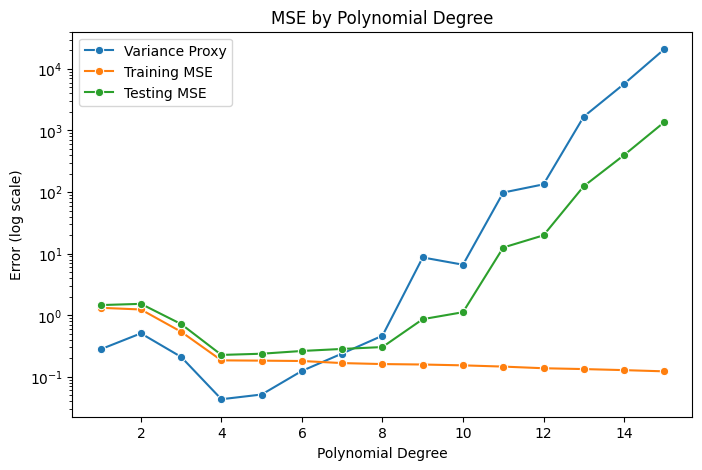
\includegraphics[width=0.6\textwidth]{../imgs/mse_graph.png} % 
		\caption{Model specs by polynomial degree}
	\end{figure}

\end{homeworkProblem}

\begin{homeworkProblem}
	\subsection{3.1.1}
	I chose to use a basis function of degree 4, from my tests using any lower degree results in very poor results.
	My bias function is in the form:


	\[
		1, \; x_1, \; x_2, \; \dots, \; x_1^4, \; x_1^3 x_2, \; \dots, \; x_2^4
	\]
	\[
		\text{Number of features } = \binom{d + \text{degree}}{\text{degree}}.
	\]

	\[
		\text{For our data we have } d = 2, \; \text{degree} = 4: \quad
		\binom{2+4}{4} = \binom{6}{4} = 15.
	\]
	\subsection{3.1.2}
	Implementing a binary classifier (for class 0) using gradient decent. I resulted a test accuracy of \textbf{97.3\%}
	\subsection{3.1.3}
	To implement a multi-class classifier you will utilize the one vs. all method. With this we will create
	n (n = \# of classes) classifiers and choose the one with the highest output.
	\subsection{3.1.4}
	\textbf{Final Multi-class Test Accuracy: 98.6\%}
	\subsection{3.2.1}
	I used the RBF kernel function to map this data.

	\[
		K(x, z) = \exp\!\left(-\frac{\lVert x - z \rVert^2}{2\sigma^2}\right)
	\]
	\subsection{3.2.4}
	\textbf{Final SVM Test Accuracy: 99.3\%}

\end{homeworkProblem}

\end{document}
